\section{Analysis}
\begin{figure*}
    \centering
    % 第一个子图及图注
    \begin{subfigure}[t]{0.32\textwidth}  % 宽度调整为页面宽度的 32%
        \centering
        \resizebox{\textwidth}{!}{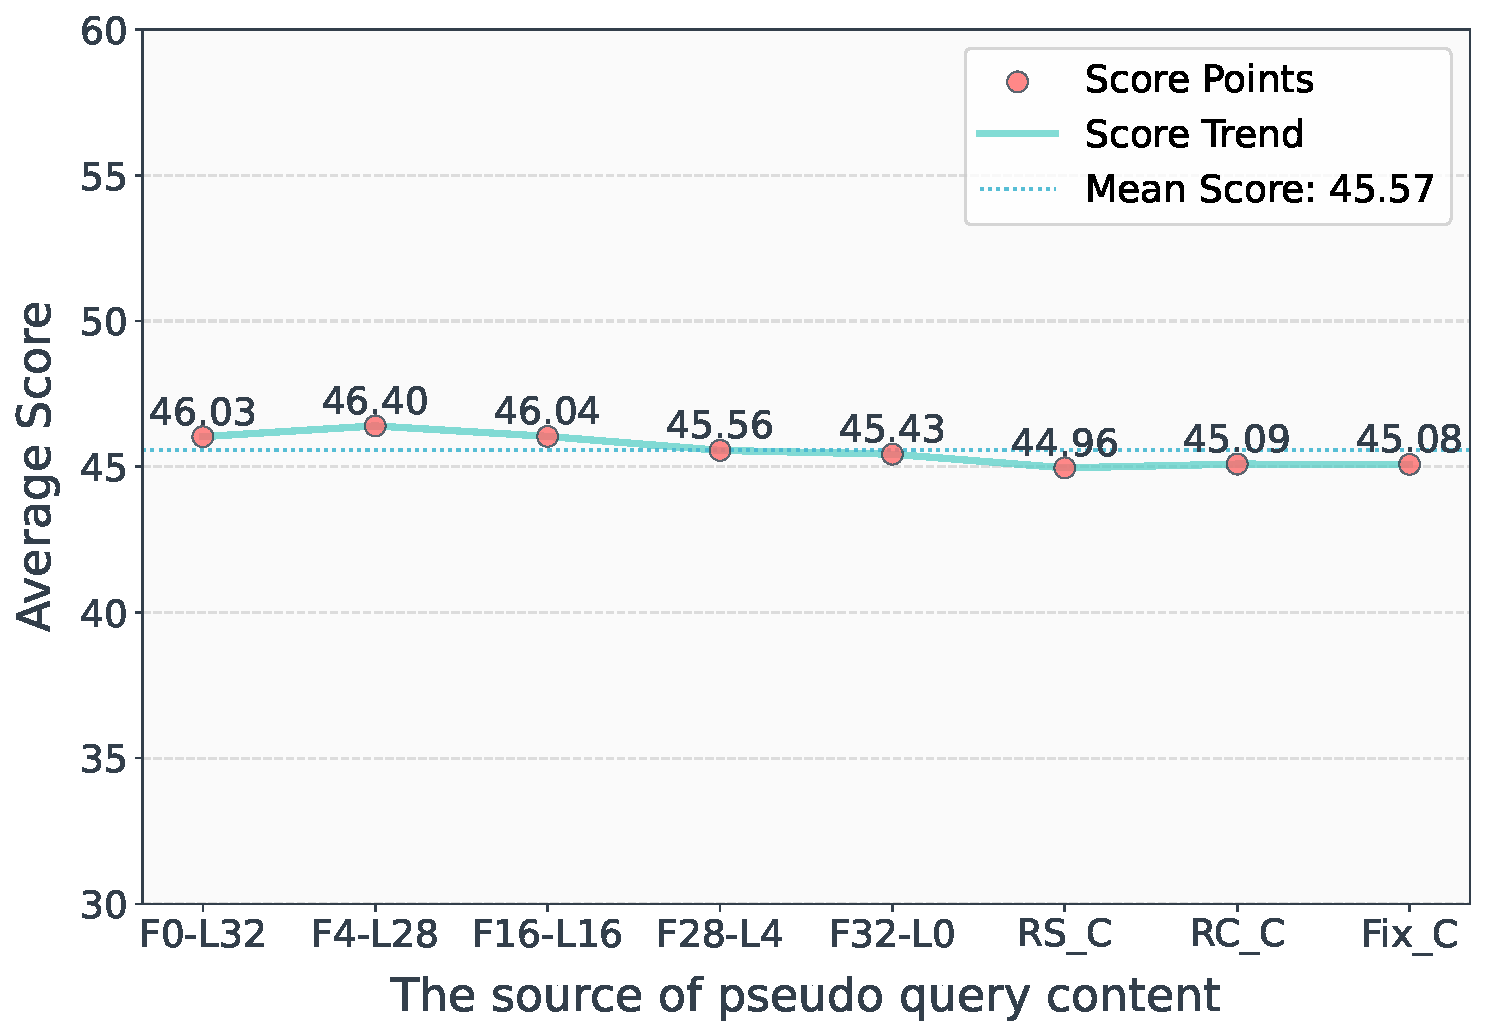
\includegraphics{images/context.pdf}}  % 适应子图宽度
        \vspace{-18pt}
        \caption{The Impact of \texorpdfstring{\(Q_{\text{pseudo}}\)}{Q\_pseudo} Quality}  % 子图图注1
        \label{fig:query_quality}
    \end{subfigure}
    \hfill  % 自动填充间距，使图片均匀分布
    % 第二个子图及图注
    \begin{subfigure}[t]{0.32\textwidth}
        \centering
        \resizebox{\textwidth}{!}{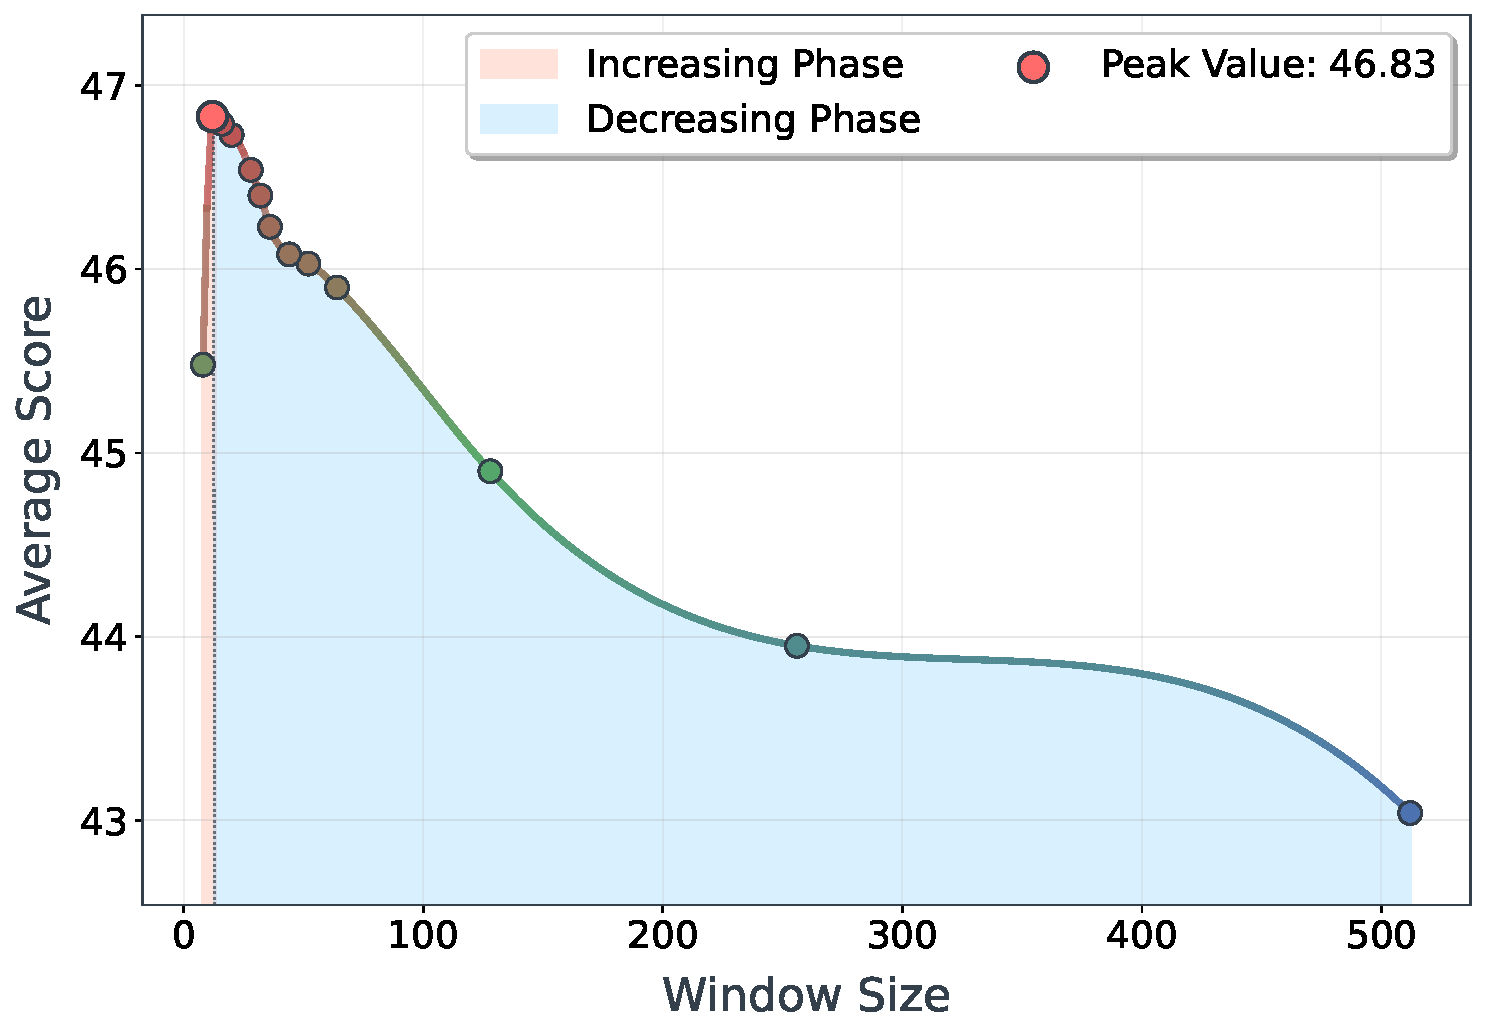
\includegraphics{images/window.pdf}}  % 适应子图宽度
        \vspace{-18pt}
        \caption{The Impact of \texorpdfstring{\(Q_{\text{pseudo}}\)}{Q\_pseudo} Length}  % 子图图注1
        \label{fig:query_length}
    \end{subfigure}
    \hfill  % 自动填充间距
    % 第三个子图及图注
    \begin{subfigure}[t]{0.32\textwidth}
        \centering
        \resizebox{\textwidth}{!}{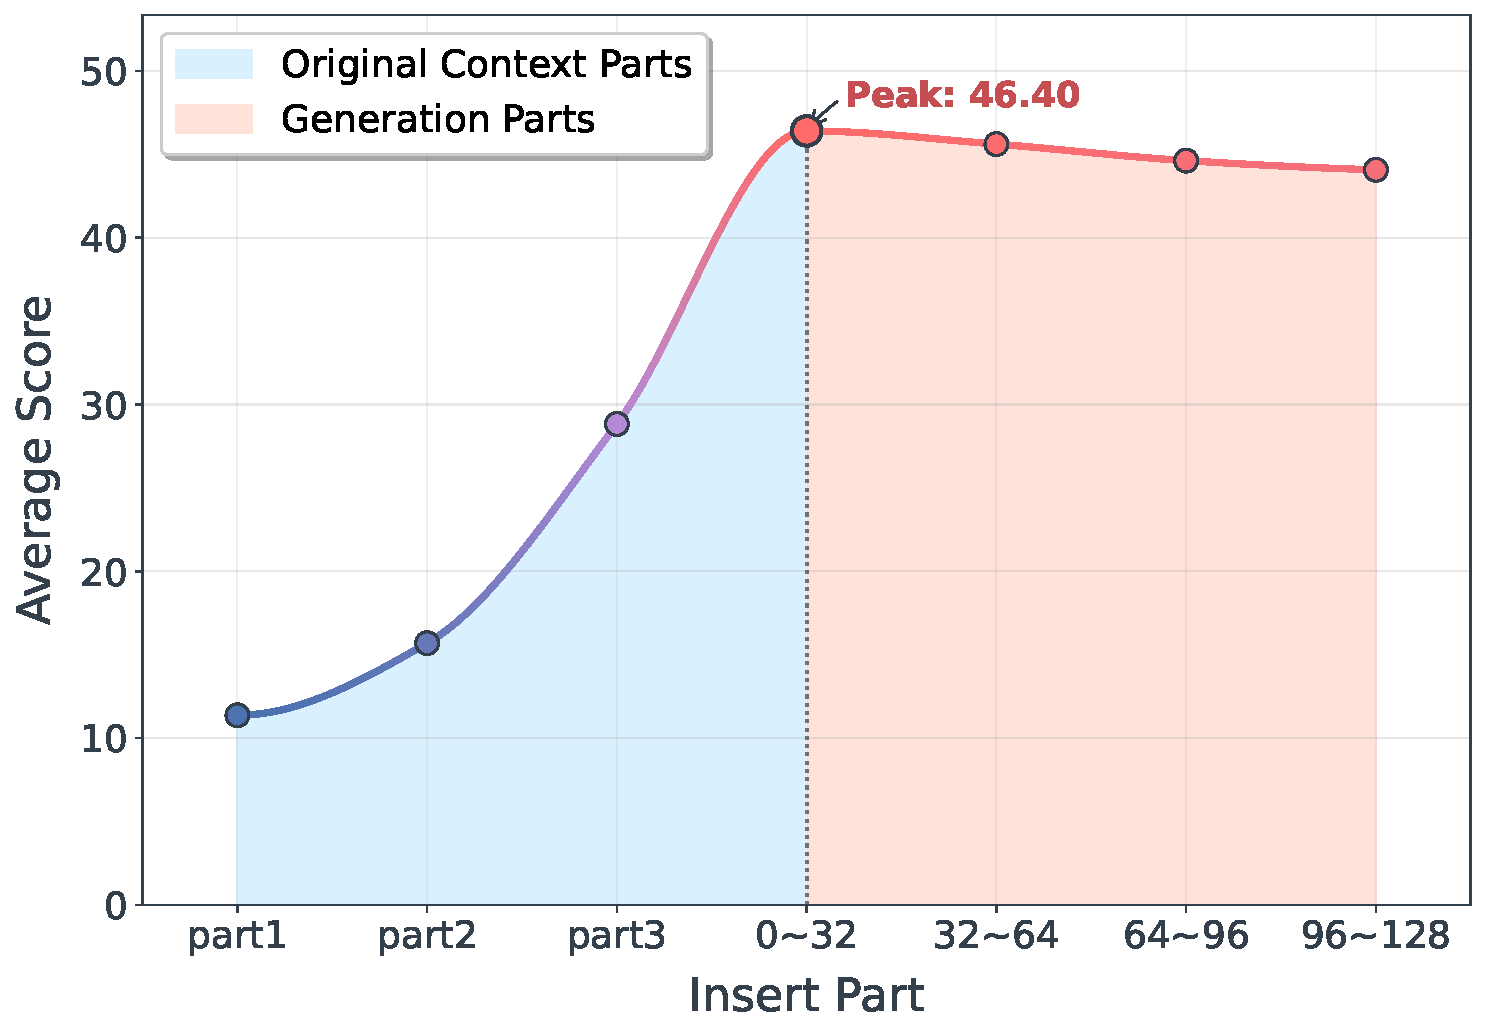
\includegraphics{images/insert_part.pdf}}  % 适应子图宽度
        \vspace{-18pt}
        \caption{The Impact of \texorpdfstring{\(Q_{\text{pseudo}}\)}{Q\_pseudo} Insert Part}  % 子图图注1
        \label{fig:query_position}
    \end{subfigure}
    % 可选：添加总标题（如需概括两图，可保留；无需则删除）
    \vspace{-7pt}
\caption{Ablation analysis of pseudo queries with respect to quality, length and insert positions. (a) Performance under a fixed \texorpdfstring{\(Q_{\text{pseudo}}\)}{Q\_pseudo} length $32$, with varying semantic content of \texorpdfstring{\(Q_{\text{pseudo}}\)}{Q\_pseudo}: \texttt{Fm\_Ln} is the concatenation of the first \texttt{m} and the last \texttt{n} tokens from the input context; \texttt{RS\_C} is constructed by concatenating 32 randomly sampled individual tokens from the context; \texttt{RC\_C} is a randomly sampled consecutive span of 32 tokens from the context; and \texttt{Fix\_C} is a fixed, repetitive nonsensical sequence (e.g., \enquote{Sorry, I don't know. Sorry, I don't know…}). (b) Performance under varying observation window sizes $N$. (c) Performance under varying insert positions of \texorpdfstring{\(Q_{\text{pseudo}}\)}{Q\_pseudo}. Left Parts: we divide the original context interval $[0, L_p)$ equally into three segments: \texttt{part1} (beginning), \texttt{part2} (middle), and \texttt{part3} (end). For each segment, we randomly select a continuous sequence of 32 positions and map the position IDs of \texorpdfstring{\(Q_{\text{pseudo}}\)}{Q\_pseudo} to it.
Right Parts: we only move backwards the position IDs of \texorpdfstring{\(Q_{\text{pseudo}}\)}{Q\_pseudo} to continuous 32 positions at different offsets after the context $L_p$ (e.g., $[L_p+0, L_p+32)$), $[L_p+32, L_p+64)$).}
    \vspace{-14pt}
\end{figure*}






\subsection{The Impact of \texorpdfstring{\(Q_{\text{pseudo}}\)}{Q\_pseudo} Semantic Content} 
 To further investigate the practical impact of semantic variation on KV cache compression performance, we conduct an ablation study by evaluating DapQ under a fixed cache budget while altering the semantic content of pseudo queries. As shown in Figure \ref{fig:query_quality}, the average performance remains highly stable (e.g., coefficient of variation $\approx 1\%$), regardless of whether the pseudo-query window is constructed from different semantic contents (e.g., the input's prefix and suffix, random in-context tokens, or nonsensical sequences). This consistency provides compelling empirical evidence that the attention pattern relies significantly on positional information to establish importance distribution, rendering the semantic content a secondary factor.



\subsection{The Impact of \texorpdfstring{\(Q_{\text{pseudo}}\)}{Q\_pseudo} Length}
The length of pseudo queries (the size of an observation window, $N$) is a crucial hyper-parameter, controlling the breadth of the simulated decoding context used for importance estimation. Figure \ref{fig:query_length} reveals a non-monotonic relationship between $N$ and performance, characterized by distinct increasing and decreasing phases.


\textbf{Increasing Phase (Small $N$):} For small window sizes, performance increases sharply as $N$ grows. This is because a small window lacks the contextual breadth to robustly estimate the importance of all relevant tokens, causing high uncertainty in the importance assessment. Adding more pseudo queries can provide a more comprehensive simulation of the decoding process, leading to a more accurate and holistic importance distribution. This expanded window thereby enables the model to identify and retain a greater number of critical tokens for future effective generation.


\textbf{Decreasing Phase (Large $N$):} Beyond a certain point, further increasing $N$ leads to a performance decline. We attribute this to a dilution effect: while initial queries in the window are precisely aligned with the start of decoding, later queries represent increasingly speculative future positions. The attention pattern for these distant positions becomes progressively diffuse and attends to tokens less relevant for initial generation steps, introducing noisier and less reliable signals into the aggregated importance scores. And mutual attention among these queries introduces additional interference, further diverting the focus from critical tokens.


This analysis identifies that the window should be sufficiently sized to capture a representative decoding context but not so large as to dilute the attentional signal. The existence of this optimum further confirms that our method is not relying on a brute-force approach. Instead, it performs a precise and efficient simulation by concentrating on the most relevant segment of the decoding trajectory.



\subsection{The Impact of \texorpdfstring{\(Q_{\text{pseudo}}\)}{Q\_pseudo} Insert Positions}

We observe that deviating from the proposed \texorpdfstring{\(Q_{\text{pseudo}}\)}{Q\_pseudo} placement (i.e., immediately following the prompt) leads to performance degradation. This phenomenon can be explained by two key factors.

\textbf{Insufficient context visibility when inserted within the context:} Under the standard causal attention mask, \texorpdfstring{\(Q_{\text{pseudo}}\)}{Q\_pseudo} placed at position $t$ can only attend to the prefix $[0, t)$ and is unable to access the subsequent context. This conflicts with our goal that \texorpdfstring{\(Q_{\text{pseudo}}\)}{Q\_pseudo} should approximate the attention patterns over the full context as seen by future decoding steps. Consequently, as shown in the left part of Figure~\ref{fig:query_position}, \texorpdfstring{\(Q_{\text{pseudo}}\)}{Q\_pseudo} placed earlier in the context fail to reconstruct global attention patterns and exhibit degraded performance.
% \textbf{Insufficient context visibility when inserted within the context:} Under the standard causal attention mask, \texorpdfstring{\(Q_{\text{pseudo}}\)}{Q\_pseudo} placed at position $t$ can only attend to the prefix $[0, t)$ and is unable to access the subsequent context. This conflicts with our goal that "\texorpdfstring{\(Q_{\text{pseudo}}\)}{Q\_pseudo} should approximate the attention patterns over the full context as seen by future decoding steps." Consequently, \texorpdfstring{\(Q_{\text{pseudo}}\)}{Q\_pseudo} inserted earlier in the context (e.g., part1 or part2) suffer from severely incomplete context visibility. They can only model local segments and are inherently unable to reconstruct global attention patterns based on the complete context, resulting in degraded performance.

\textbf{The assigned position of \texorpdfstring{\(Q_{\text{pseudo}}\)}{Q\_pseudo} shifts backwards away from the correct interval, introduces increasing misalignment in the RoPE embedding space.} Large backward shifts in positions lead to accumulated rotational offsets, causing the \texorpdfstring{\(Q_{\text{pseudo}}\)}{Q\_pseudo} representation space to progressively diverge from those of real queries. This misalignment makes it harder for \texorpdfstring{\(Q_{\text{pseudo}}\)}{Q\_pseudo} to approximate the target attention distribution, explaining the observed performance drop with larger positional shifts, as clearly illustrated in the right part of Figure~\ref{fig:query_position}.